\chapter{Modelagem Arquitetural}

Apresentamos abaixo a modelagem arquitetural do sistema de delivery, utilizaremos para nossa modelagem o modelo C4.

\section{Diagrama de Contexto}
Começaremos pelo diagrama de contexto, nele temos o nosso sistema de delivery Pop Food que é
responsável por gerenciar todo o estabelecimento, e os atores como clientes e atendentes/administradores que fazem pedido de comida
e são responsáveis pela administração dentro do software respectivamente. Podemos verificar ainda 
os sistemas externos como PagSeguro e Ifood para pagamento e pedidos online respectivamente.
\begin{figure}[h]
    \centering
    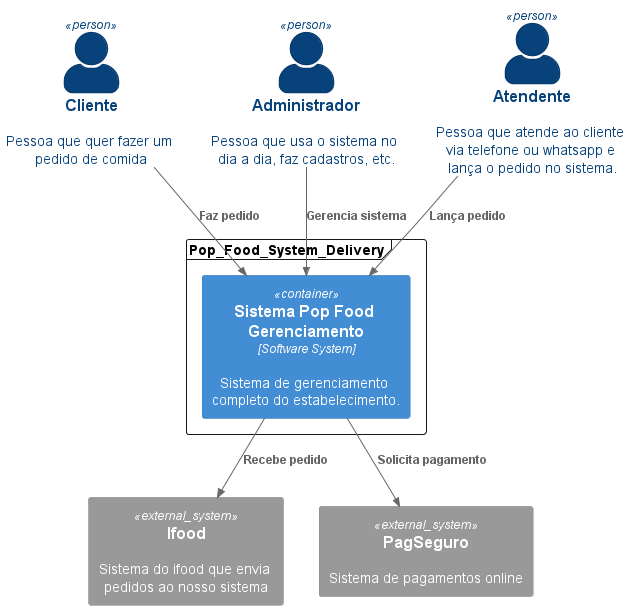
\includegraphics[width=1\textwidth]{diagrama_contexto.png}
    \caption{Diagrama de Contexto}
    \label{fig:Diagrama de Contexto}
  \end{figure}

  \href{https://github.com/soltein/TCC/blob/main/Diagramas/out/diagrama_contexto/diagrama_contexto.png}{Imagem resolução maior}

  \section{Diagrama de Container}
  Mostramos agora o diagrama de container, nele podemos observar que teremos dois containers de frontend,
  ambos utilizando a tecnologia Angular, o frontend do Cliente é responsável por apresentar as telas do sistema
  que os clientes utilizarão para se cadastrar, ver o menu de opções, efetuar pedidos e pagamentos online.

  No frontend de administração será disponibilizado as telas de login e administração do sistema, como cadastro de produtos, possibilidade de lançamento de pedidos,
  cadastro de clientes, etc.

  Neste diagrama vemos o container do back end, que utilizará spring boot e será responsável pelas regras de negócio e integração com banco de dados e sistemas externos como iFood e PagSeguro.

  \begin{figure}[h]
    \centering
    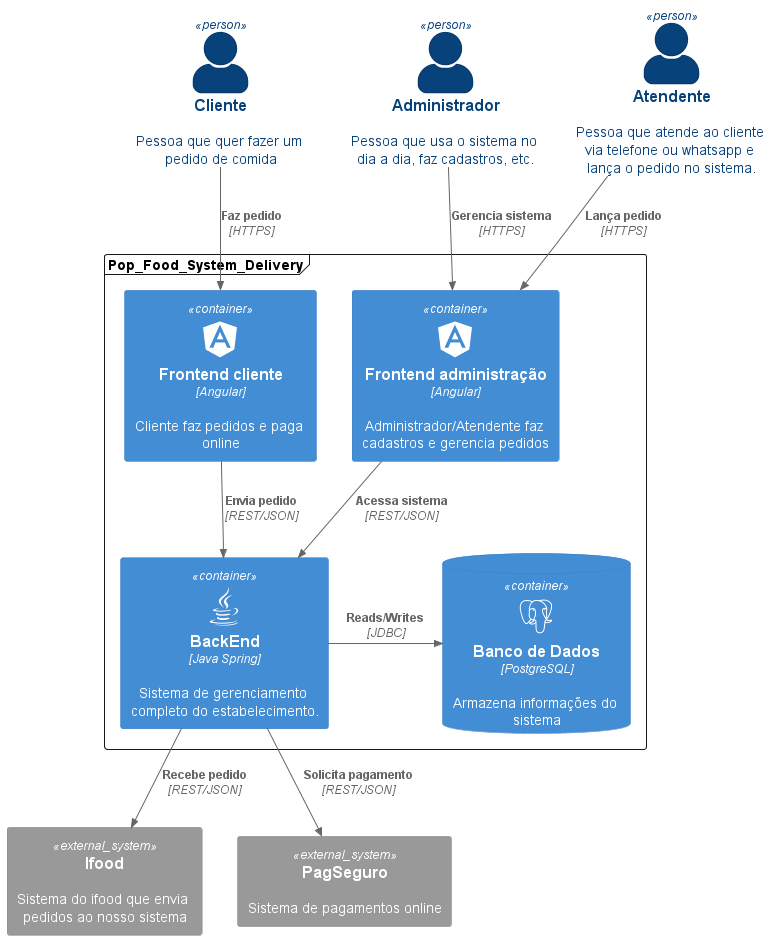
\includegraphics[width=0.9\textwidth]{diagrama_container.png}
    \caption{Diagrama de Container}
    \label{fig:Diagrama de Container}
  \end{figure}

  \href{https://github.com/soltein/TCC/blob/main/Diagramas/out/diagrama_container/diagrama_container.png}{Imagem resolução maior}

  \section{Diagrama de Componentes}
  Entrando mais em detalhes, temos agora o diagrama de componentes, nele podemos ver as abstrações em caixa preta dos principais componentes
  do sistema.
  
  \begin{figure}[h]
    \centering
    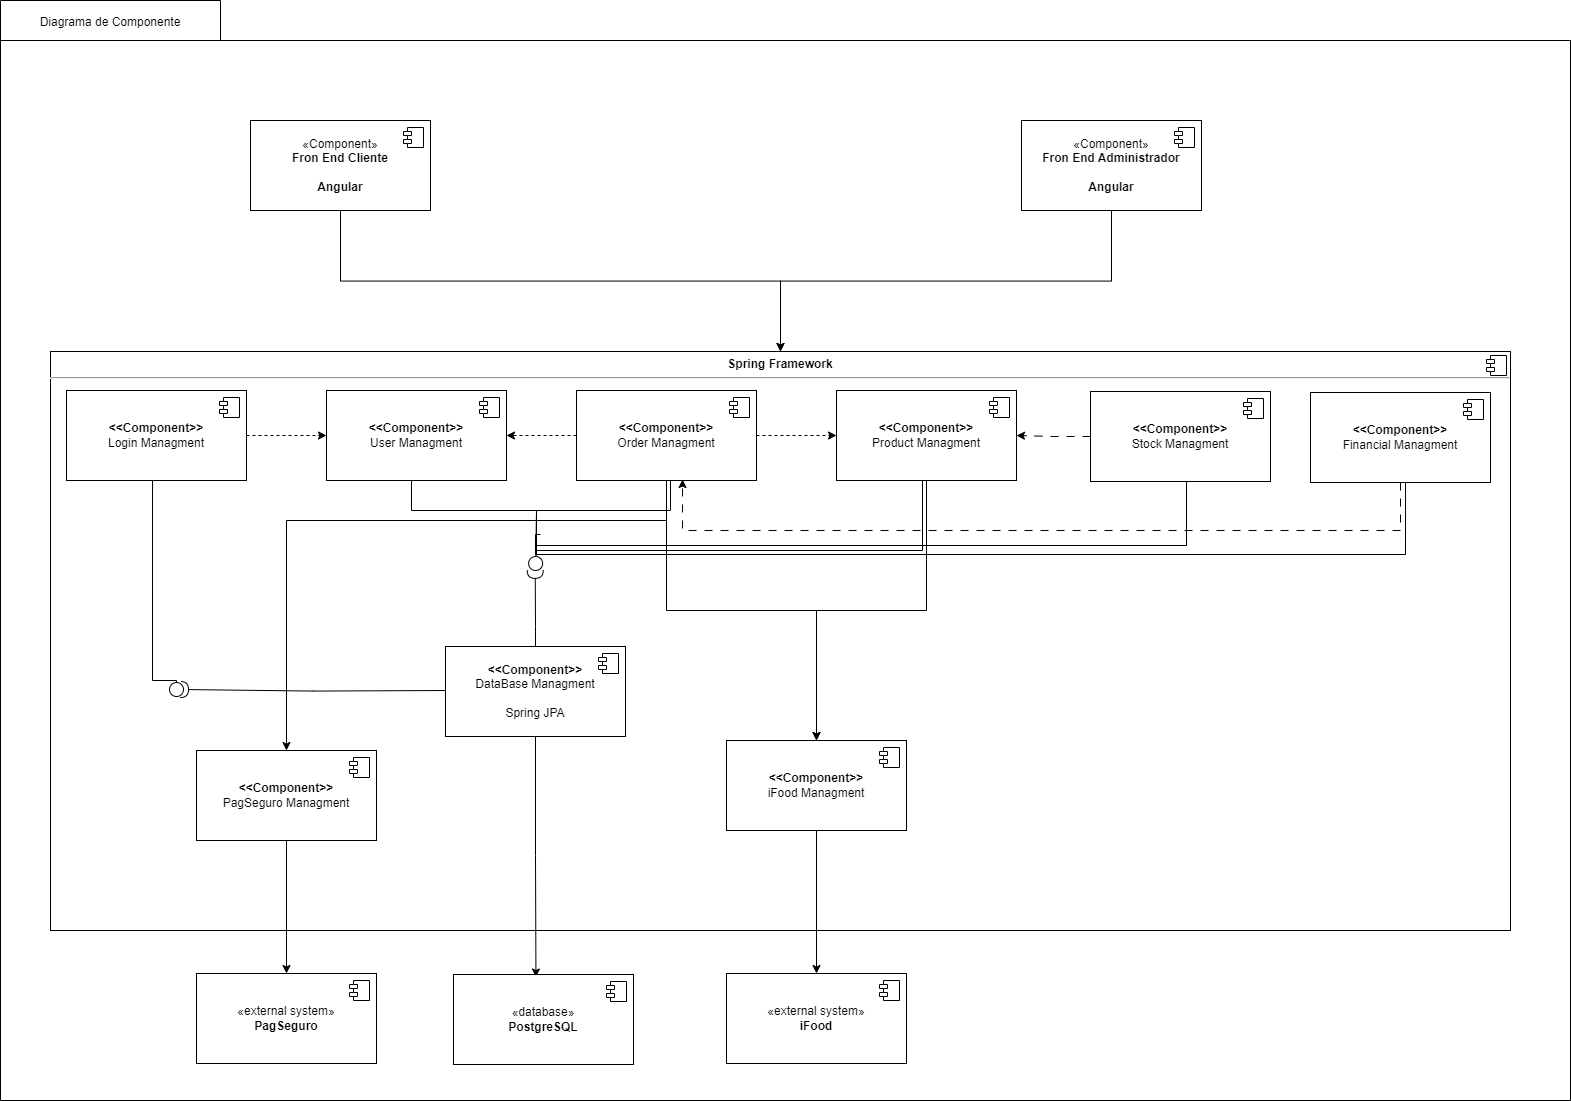
\includegraphics[width=1\textwidth]{diagrama_componentes.png}
    \caption{Diagrama de Componentes}
    \label{fig:Diagrama de Componentes}
  \end{figure}

  \href{https://github.com/soltein/TCC/blob/main/Diagramas/out/diagrama_componentes.png}{Imagem resolução maior}
